% A (little more than a) minimal working example
\documentclass[12pt, a4paper]{article}

% Increase tex widht and heigh by 4cm
\addtolength{\textwidth}{4cm}
\addtolength{\oddsidemargin}{-2cm}
\addtolength{\textheight}{4cm}
\addtolength{\topmargin}{-2cm}

% To start out let's include the following packages
\usepackage[utf8]{inputenc} % encoding
\usepackage[hidelinks]{hyperref} % for clickable references
\usepackage{xcolor} % custom colors
\usepackage{graphicx} % for including graphics
\usepackage{pgfplots} % for plots and more
\usepackage{tikz} % for drawing and more
\usepackage{booktabs} % for nice tables
\usepackage{amsmath} % math stuff
\usepackage{amsfonts}
\usepackage{amssymb}
\usetikzlibrary{calc}
\usetikzlibrary{positioning}
\usetikzlibrary{arrows.meta}
\usetikzlibrary{fit}

\begin{document}

\title{%
  {\bfseries From Ethernet to InfiniBand}\\[1ex] % your title goes here
}
\author{ Philipp Czerner} % your name

\date{\vspace{-5ex}} % dirty hack to remove date from titlepage

{\sf \maketitle} % use serif free font for title page

\begin{center}
  \includegraphics[width=8cm]{logo_sdv.pdf}\\
  {\large\sf Sommerakademie in Leysin, August 2016}
\end{center}

\vspace{1cm}

\begin{abstract}
  The interconnect is an important piece of any high-performance computing cluster. This paper presents the basics of networking technologies in general and of Ethernet and InfiniBand in particular. The advantages of the InfiniBand are discussed, with a focus on power-saving potential when used as interconnect. 
\end{abstract}

% The table of contents
\newpage
\tableofcontents

\newpage
\section{Introduction}\label{sec:introduction}
As processors continue to evolve, network technologies need to keep pace, prompting new developments to improve both latency and bandwidth. In recent times the power consumption has started to gain importance as well, as energy costs make up a significant margin of the total cost of a computing cluster. With CPUs becoming more efficient in recent years and computation increasingly parallised, interconnect technologies shape up as a significant factor of the consumed energy and a promising area for improvements.

In this paper I will give a short introduction into network technologies via the OSI model. Then both Ethernet and InfiniBand will be discussed, as the two most common interconnect technologies for high-performance computing (HPC). This includes the improvements made by InfiniBand over Ethernet, especially as related to power consumption.

\section{OSI Model}
The Open Systems Interconnection model describes and standardises the workings of a communications system. Its main concept is the \textit{layer}, of which there are seven. Each layer uses the functionality of the layer below and provides an interface to the layer above.

\begin{figure}[h]
\begin{center}
	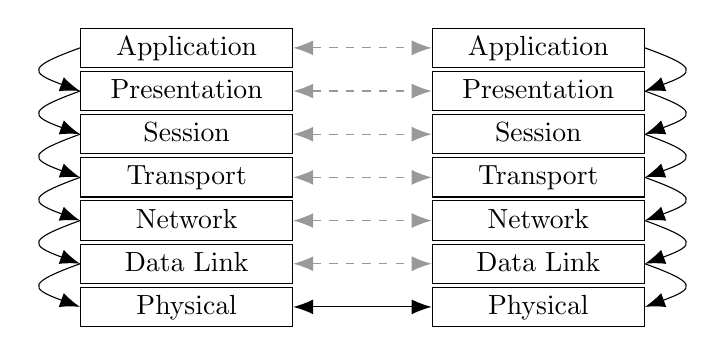
\begin{tikzpicture}[node distance=1pt,<->/.tip={Latex[scale=1.5]}]
	\tikzstyle{box}=[rectangle,align=center,draw,text height=1.5ex
	,text depth=.25ex,text width=7em]
	\tikzstyle{dashy}=[<->,dashed,color=black!40]
	
	\node[box] (n1) at (0,0) {Physical};
	\node[box] (m1) [right=5em of n1] {Physical};
	\foreach \x/\xx/\y in {2/1/Data Link,3/2/Network,4/3/Transport,5/4/Session,6/5/Presentation,7/6/Application} {
		\node[box] (n\x) [above=of n\xx] {\y};\node[box] (m\x) [above=of m\xx] {\y};}
	
	\draw[<->] (n1) -- (m1);
	\foreach \x/\y in {2/1,3/2,4/3,5/4,6/5,7/6} {\draw[dashy] (n\x ) -- (m\x );
		\draw[<-] (n\y.west) ..controls +(160:0.7cm) and +(200:0.7cm).. (n\x.west);
		\draw[<-] (m\y.east) ..controls +(20:0.7cm) and +(340:0.7cm).. (m\x.east);}
	
	\end{tikzpicture}
\end{center}
\caption{The layers of the OSI model}
\label{osilayers}
\end{figure}

Direct communication (i.e. the exchange of bits via a physical medium) only happens on layer 1 (Physical Layer), the other layers conduct virtual communication using the facilities of the respective lower layer. The OSI model specifies the following layers:

\begin{itemize}
\item Layer 1 (Physical) describes and specifies the physical medium. This includes the type of medium (wireless, copper cable, fiberoptic cable), its properties (insulation, frequencies), plugs (dimensions, pin layout), and timing.

Examples: Ethernet physical layer, DSL, SONET/SDH

\item Layer 2 (Data Link) organises a reliable transfer of data between neighbouring nodes. This includes flow control (ensuring that a faster node does not flood a slower node with data), error checking (via checksum, this detects errors during transmission with high confidence), and collision handling (when using a shared medium).

Examples: Ethernet, PPP, ATM

\item Layer 3 (Network) handles multi-node networking. It provides address translation from physical addresses (MAC address, for example), that are unique and bound to the hardware, to logical addresses (IP address, for example), that may include routing information like subnets. There is also routing (choosing the path between two nodes in the network) and traffic control (prevent the nodes from overloading the network).

Examples: IPv4, IPv4

\item Layer 4 (Transport) provides a reliable data transfer between nodes in the network. This includes acknowledging successful packets, checking data integrity using checksums and ensuring correct ordering of packets with sequence numbers.

Examples: TCP, UDP

\item Layer 5 (Session) controls the connection between the nodes. This includes initalization and termination of the connection and its mode of operation (full/half duplex or simplex). 

Examples: Sockets, RPC

\item Layer 6 (Presentation) enables independence from data representation. It converts between different formats and encrypts and decrypts the data as needed.

Examples: TLS, MIME

\item Layer 7 (Application) directly communicates with the application process, which itself is outside of the OSI model. Its functionality is application dependant.

Examples: HTTP, SSH
\end{itemize}

The internet is based on the TCP/IP stack and does not conform strictly to the specification of the OSI model. It can, however, be used as context to categorize and compare different protocol stacks. As all examples here work with the internet, they do not conform to the specification either and do not necessarily provide all features present in the layer.

\section{Ethernet}
Ethernet is a family of standards used mostly in local area networks (LANs). The standards 10BASE-T, 100BASE-TX and 1000BASE-T are commonly used in consumer hardware, with almost all motherboards directly providing a port. It is located at both the physical and the data link layer.

10BASE-T, 100BASE-TX and 1000BASE-T are based on shielded twisted pair cabling and have data rates of 10, 100 and 1000 Mbit/s, respectively, but there are other standards for different transmission mediums (fibreoptic cabling, for example) allowing for data rates as high as 100 Gbit/s.

Gigabit Ethernet, as well as 10G (10 Gbit/s) and 40G (40 Gbit/s) Ethernet, are also used as interconnect in HPC, making up 44\% of the computer in the Top500 list (as of June 2016) \cite{top500list}. This makes Ethernet the most used interconnect family.

Ethernet is commonly used together with the protocols IP (Internet Protocol) and TCP (Transmission Control Protocol). IP is located at layer 3 (network) of the OSI model, TCP at layer 4 (transport). As Ethernet does not provide error handling by itself, TCP ensures the correctness of data.

\section{InfiniBand}
InfiniBand (IB) is a networking technology with a focus on high bandwidth and low latency. Similar to Ethernet, it consists of multiple standards. IB is used in HPC as interconnect and was utilized by 41\% of systems in the Top500.

The functionality provided by IB spans the first four layers of the OSI model, which makes protocols like TCP or IP unnecessary. They can, however, be mapped onto IB, which enables application to access IB via a more traditional API.

\subsection{Architecture}
IB's equivalent of a network interface controller (NIC) is called \textit{host channel adapter} (HCA). The HCA is usually installed in the form of a PCI Express card, in contrast to Ethernet, which is often directly integrated into the motherboard.

The HCA provides the functionality of layers 1-4 in hardware. This includes all time-critical functionality (such as sending and receiving data), but does not extend to \textit{all} of IB's features. Ethernet does not provide layer 3 and 4 functionality by itself, but relies on TCP and IP, which are software-based protocols.

IB provides both send/receive and RDMA based communication, both either reliable or unreliable. Send/receive is the traditional mode of network communication, featuring a stream of data that is sent from one end and received at the other. RDMA is described in detail in the next section. Reliable communication gurantees correctness of data, meaning that no data is lost, duplicated or changed during the transfer. Some applications may, however, value the reduced overhead more than error-free data (video streaming, for example), especially in the context of LANs, where errors are rare due to short distances and controlled conditions.

\textit{Work Queue Requests} (WQR) specify some work for the HCA to do, this may be a send/receive or RDMA request. These are organised into two queues, the send and the receive queue, which form the \textit{Queue Pair} (QP).

\subsection{RDMA}
Remote Direct Memory Access (RDMA) is a technique to efficiently transfer data over the network, with minimal latency and processing overhead.

Traditionally, an application sends data over the network by calling an appropiate function of the kernel. Then the data is copied into a buffer managed by the kernel and the NIC is notified to send the data over the network to the other node, where this process happens in reverse.

Using RDMA there is no middle step: The application notifies the HCA to write the data over the network, then the HCA reads the data directly and asynchronously off the application's memory and transfers it. The other node's HCA receives the data and writes it into the remote application's memory space.

There is no intermediate copy, making it a zero-copy transfer. Neither the local nor the remote CPU are involved in the process of transmitting the data. When reading data from a remote source, the remote CPU is not involved at all. Additionally the application does not call into the kernel, saving the CPU from doing expensive context switches.

Memory on modern machines is virtualised, meaning that each access from a user-level application goes through an indirection that maps it to the physical address. The kernel manages this mapping. An HCA does not have the same limitations as a user-level program, meaning that additional measures have to be taken to ensure memory safety. To initiate an RDMA request the application needs to register the memory regions first via the kernel, which checks whether the addresses are valid and translates them into physical addresses for the HCA. A key for this memory region is returned, which is needed to start any RDMA request involving this region (both locally and remotely).

\subsection{Advantages}
The kernel is not involved in any time sensitive operations; this eliminates the need for context switches and improves the latency. When using RDMA, there is minimal to none utilization of the CPU as well, enabling it to spend more time on the calculations as opposed to IO. This is aided by the hardware-based approach of IB, where the networking logic is offloaded onto custom and thus optimised circuits.

\subsection{Power Consumption}
The power consumption of an HPC cluster is a significant chunk of its operating costs, which in turn make up a large part of the total cost. Efforts to reduce power consumption have been made, but the interconnects have received little attention as of now.

On some HPC systems the interconnect consumes 15-20\% of the total idle power, this percentage is expected to scale as the cluster become larger \cite{hoefler2010software}.

The main advantage of IB in terms of power consumption is its lower CPU overhead, achieved both by implementing the network stack in hardware and utilizing RDMA.

It is the interconnect of choice for many systems in the Green500 (as of June 2016), where it is used by 48\% of the top 100 systems, with 17\% using Ethernet \cite{green500list}. (Comparing the full Green500 does not yield very interesting results, as it is mostly a permutation of the Top500.) For comparision, 41\% and 44\% of systems in the Top500 use IB and Ethernet, respectively.

\section{Further Reading}
\cite{hoefler2010software} discusses different options for power saving in HPC interconnects. \cite{Rodiger2015HQ} gives a more in-depth overview of the workings of IB and its potential for improved performance in the context of database query processing. \cite{abts2010energy} describes techniques for improving the energy efficiency of datacenters via adaptations of the networking technology.

% References
\bibliographystyle{plain}  % you can try 'alpha' or 'abbrv' instead of 'plain'
\bibliography{paper} % references are found in the file `paper.bib`

\end{document}
